%% 
%% Correspondence to: Baizid MD Ashadzzaman, Department of Computer
%% Science and Engineering, International Islamic University Chittagong,
%% Chittagong, Bangladesh.
%%
\documentclass[a4paper,fleqn]{cas-dc}

\usepackage[numbers]{natbib}
\usepackage{subcaption}
\usepackage{float}

%%%Author definitions
\def\tsc#1{\csdef{#1}{\textsc{\lowercase{#1}}\xspace}}
\tsc{BEC}
\tsc{SE}
%%%

\begin{document}
\let\WriteBookmarks\relax
\renewcommand\topfraction{.85}
\renewcommand\textfraction{.15}
\renewcommand\bottomfraction{.7}
\renewcommand\dbltopfraction{.9}
\renewcommand\floatpagefraction{.75}
\renewcommand\dblfloatpagefraction{.85}
\setcounter{topnumber}{3}
\setcounter{bottomnumber}{2}
\setcounter{totalnumber}{5}
\setcounter{dbltopnumber}{2}
\shorttitle{Attention-based waste classification for environmental sustainability}
\shortauthors{B.M. Ashadzzaman}

\title [mode = title]{Enhanced Waste Classification Using an Attention-Based Neural Network with Grad-CAM Interpretability for Environmental Sustainability}

\author[1]{Baizid MD Ashadzzaman}[orcid=0009-0008-4137-5905]
\cormark[1]
\ead{baizid.md.ashadzzaman@gmail.com}

\credit{Conceptualization, Methodology, Software, Validation, Formal analysis,
Investigation, Data curation, Writing -- original draft, Writing -- review and editing}

\cortext[cor1]{Corresponding author}
\affiliation[1]{organization={Department of Computer Science and Engineering, International Islamic University Chittagong},
city={Chittagong},
state={Chittagong},
country={Bangladesh}}

\begin{abstract}
Effective municipal solid-waste management depends on the accurate and timely
identification of heterogeneous waste streams. Yet automated waste-sorting
systems that are trained on pristine, non-contaminated object images frequently
fail when deployed under real landfill conditions, where materials are
contaminated, deformed, mixed, and visually ambiguous. In this work, we propose
an attention-guided transfer-learning framework for nine-class waste
classification using the RealWaste dataset, a collection of 4{,}752 RGB images
acquired at an operating landfill site. The framework couples a frozen
DenseNet-121 backbone with a lightweight channel-attention gate that
recalibrates the final feature maps using global average and maximum pooling
followed by a two-layer perceptron and sigmoid gating. Only the attention
module and the classifier head are trained, using class-weighted
cross-entropy to counteract the pronounced label imbalance, the Adam
optimiser, an adaptive learning-rate scheduler, and early stopping. A
stratified 70/15/15 train--validation--test split preserves class
distributions across all partitions. The proposed model reaches a test
accuracy of 82.35\% with a macro-averaged precision, recall and $F_1$-score of
0.83, outperforming six competing backbones (ResNet-50, MobileNetV2, VGG-16,
Inception-V3, Inception-ResNet-v2, and a compact custom CNN) under an
identical evaluation protocol. An ablation study confirms that the channel
attention module raises the accuracy of the DenseNet-121 baseline from
79.41\% to 82.35\% and improves the macro-$F_1$ from 0.80 to 0.83, with the
largest gains observed for the visually similar Plastic and Miscellaneous
categories. Gradient-weighted class activation maps (Grad-CAM) provide
post-hoc interpretability, confirming that the model attends to salient waste
objects rather than irrelevant background. The proposed pipeline offers an
accurate, transparent, and reproducible baseline for automated landfill waste
sorting and recycling automation.
\end{abstract}

\begin{keywords}
Waste classification \sep Attention mechanism \sep DenseNet-121 \sep Transfer learning
\sep Channel attention \sep Grad-CAM \sep RealWaste \sep Deep learning
\end{keywords}

\maketitle

%% ---------------------------------------------------------------
\section{Introduction}\label{sec:intro}

Waste management has become one of the most pressing environmental challenges
of the modern era. Rapid urbanisation, industrialisation and growing
consumerism have driven an unprecedented increase in the volume of municipal
solid waste, and the way in which this waste is sorted and treated directly
determines recycling rates, landfill dependency, public health and
environmental sustainability~\cite{realwaste}. Conventional sorting
strategies based largely on manual inspection or on rigid rule-based
policies are labour-intensive, slow, subjective, and notoriously
error-prone. Misclassification at the source propagates through the entire
recycling chain: contaminated batches are rejected, valuable recyclables are
lost to landfill, and recovery efficiency drops~\cite{trashnet,meng_a_study}.

Recent advances in deep learning, and in convolutional neural networks (CNNs)
in particular, have established image classification as a mature technology
capable of end-to-end feature learning from raw pixels~\cite{simonyan_vgg,he_resnet,huang_densenet}.
When applied to waste recognition, CNNs have repeatedly demonstrated their
superiority over hand-crafted-feature pipelines, for example HOG+SVM
set-ups~\cite{meng_a_study}. However, most published waste-classification
systems are trained and evaluated on \emph{pristine} or synthetic datasets
such as TrashNet~\cite{trashnet}, whose objects are photographed in clean,
controlled conditions. Such models, which can reach very high accuracy in the
laboratory, deteriorate sharply when confronted with the messy, contaminated,
deformed and overlaid items that arrive continuously at real landfill
sites~\cite{realwaste,deepwaste}. The same models also behave as opaque
black boxes, offering no explanation for their predictions, which limits
their deployment in regulated industrial settings where transparency is
expected~\cite{selvaraju_gradcam}.

These two shortcomings poor generalisation to authentic waste streams and
the absence of interpretability motivate the present study. We build upon
three established pillars. First, we adopt transfer learning, which reuses
feature representations learned on large-scale natural-image corpora
(ImageNet) and adapts them to the target domain with comparatively few
labelled examples~\cite{pan_transfer}. Second, we augment the transferred
backbone with a \emph{channel attention} mechanism, a lightweight
recalibration operator inspired by the Squeeze-and-Excitation
architecture~\cite{hu_senet} and the convolutional block attention
module~\cite{woo_cbam}, which allows the network to emphasise the feature
channels that are most informative for distinguishing visually similar waste
materials. Third, we attach gradient-based visual explanations
(Grad-CAM)~\cite{selvaraju_gradcam} so that every decision can be inspected
at the pixel level. Figure~\ref{fig:schema} summarises this end-to-end
framework schematically.

Concretely, the paper makes the following contributions:
\begin{itemize}
\item We design and implement an attention-guided waste-classification
framework built on a frozen DenseNet-121 backbone~\cite{huang_densenet} with a
channel-attention gate and a custom classifier head, trained end-to-end on the
RealWaste dataset with class-weighted cross-entropy, an adaptive learning-rate
scheduler and early stopping.
\item We provide a controlled comparison of the proposed framework against
six alternative transfer-learning backbones ResNet-50~\cite{he_resnet},
MobileNetV2~\cite{sandler_mobilenet}, VGG-16~\cite{simonyan_vgg},
Inception-v3~\cite{szegedy_inceptionv3}, Inception-ResNet-v2~\cite{szegedy_inceptionresnet},
and a compact custom CNN under an identical data pipeline and optimisation
protocol.
\item We conduct an ablation study that isolates the effect of the channel
attention module, and we analyse the failure modes of the model with
confusion matrices and per-class metrics.
\item We use Grad-CAM heatmaps to verify that the trained model focuses its
predictions on salient waste objects, providing a principled and transparent
basis for deployment in recycling and landfill-sorting facilities.
\end{itemize}

The remainder of the paper is organised as follows.
Section~\ref{sec:related} reviews related work on waste classification,
attention mechanisms and explainability.
Section~\ref{sec:methods} describes the dataset, the proposed architecture,
the channel-attention formulation, and the training and evaluation strategy,
together with the underlying mathematical formulations.
Section~\ref{sec:results} reports and discusses the experimental results,
including the backbone comparison, the attention ablation, confusion-matrix
analysis and Grad-CAM interpretations.
Section~\ref{sec:conclusion} concludes the paper and outlines directions for
future work.

\begin{center}
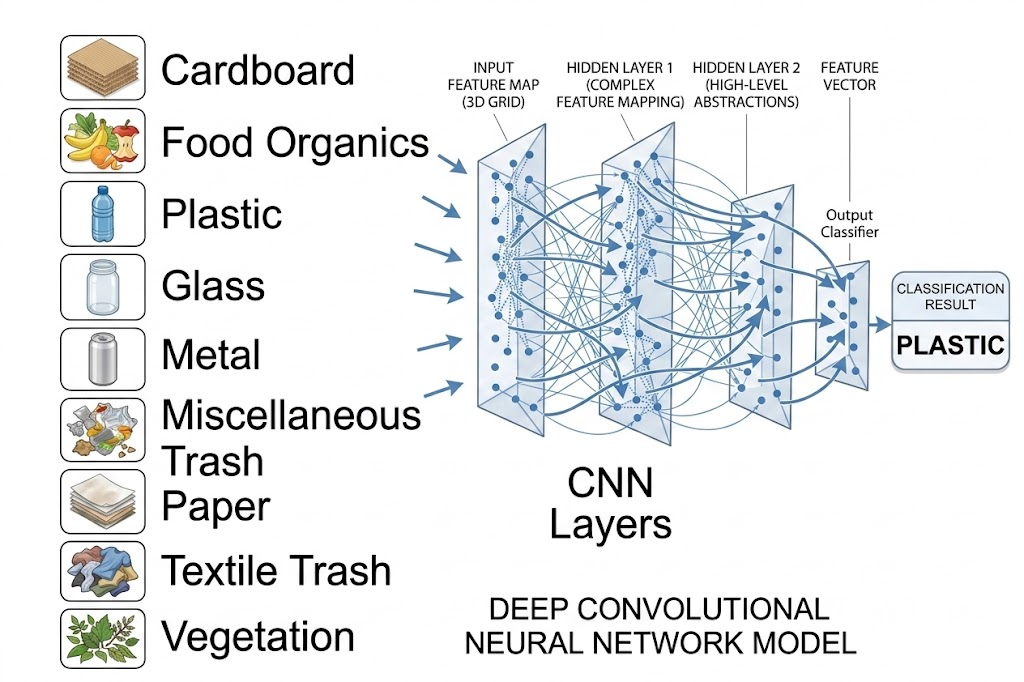
\includegraphics[width=0.9\linewidth]{figures/fig1_schematic.jpg}
\end{center}
\captionof{figure}{High-level overview of the attention-guided waste-classification
framework. Raw landfill images are preprocessed, encoded by a frozen
ImageNet-pretrained CNN, recalibrated by a channel-attention gate, and mapped
to class probabilities by the classifier head. For every prediction a
Grad-CAM heatmap can be produced for inspection.}
\label{fig:schema}

\section{Related Work}\label{sec:related}

\subsection{Waste classification with deep learning}

Early automated waste-recognition systems relied on hand-crafted features
combined with classical classifiers; for example, Meng and Chu~\cite{meng_a_study}
compared histogram-of-oriented-gradients (HOG) descriptors with support
vector machines against CNN classifiers and showed that deep models, in
particular ResNet-50 with data augmentation, clearly outperformed the
classical pipeline. Wang demonstrated a four-class VGG-16 system with batch
normalisation and ReLU activations that reached roughly 75\% accuracy,
illustrating both the promise and the limitations of early CNN-based
sorters. Recognising the constraints of embedded hardware, Rabano
et~al.~\cite{rabano_common} retrained MobileNet via transfer learning on the
TrashNet dataset and reported 87.2\% accuracy in a mobile Android
application, establishing the feasibility of on-device real-time waste
classification. Aral et~al.~\cite{aral_trashnet} benchmarked several modern
CNNs on TrashNet, while Bashkirova et~al.~\cite{deepwaste} proposed
DeepWaste, a deep network for fine-grained waste material classification.

A recurring limitation in this literature is the dataset itself. Most
benchmarks, TrashNet included, contain clean, single-object photographs that
do not reflect the comingled, contaminated and deformed waste streams found
in operating landfills. The RealWaste dataset~\cite{realwaste} was
specifically collected at the Whyte's Gully Waste and Resource Recovery
Centre (Wollongong, Australia) to close this gap, and its authors showed
that models trained on pristine material datasets lose more than 30
percentage points of accuracy when transferred to authentic landfill images.
These findings motivate the use of RealWaste and of training protocols that
are robust to label imbalance and visual ambiguity in the present study.

\subsection{Attention mechanisms in convolutional networks}

Attention mechanisms, originally introduced for sequence modelling in the
Transformer architecture~\cite{vaswani_attention}, have been adapted to
computer vision in a variety of forms. The Squeeze-and-Excitation (SE)
block~\cite{hu_senet} performs channel-wise recalibration by squeezing each
feature map with global average pooling and using two fully connected layers
to produce per-channel gating weights. The convolutional block attention
module (CBAM)~\cite{woo_cbam} extends this idea by combining both channel and
spatial attention and by fusing average- and max-pooled descriptors. These
modules add only a small number of parameters while consistently improving
discriminative power, which is precisely the behaviour needed for waste
categories that share texture, colour and shape (e.g.\ plastic versus glass,
or plastic film versus metal foil). Recent waste-classification studies have
confirmed that attention-augmented variants of EfficientNet and DenseNet
deliver higher recognition accuracy at a lower computational cost, and that
they generalise better to small heterogeneous benchmarks. In this work we
adopt a channel-attention gate, defined formally in
Section~\ref{sec:channel-attention}, which combines average and maximum
pooling before a two-layer perceptron with sigmoid gating.

\subsection{Interpretability for image classifiers}

Beyond accuracy, industrial adoption of automated sorting requires that model
decisions be auditable. Gradient-weighted class activation
mapping~\cite{selvaraju_gradcam} produces class-specific saliency heatmaps by
weighting the last convolutional feature maps with the global-average-pooled
gradients of the predicted class score. Grad-CAM has been widely used to
verify that classifiers localise the objects they claim to recognise and to
diagnose systematic biases such as reliance on background cues or on
contaminants. In the waste-classification context, Grad-CAM can reveal
whether a model correctly attends to the waste object itself or is misled
by stains, reflections, or neighbouring items and thereby provides an
actionable tool for model auditing and for trust in the deployed system.

\section{Materials and Methods}\label{sec:methods}

\subsection{Problem formulation}

Let $\mathcal{D}=\{(\mathbf{x}_n, y_n)\}_{n=1}^{N}$ denote a labelled dataset
of waste images, where $\mathbf{x}_n \in \mathbb{R}^{3\times H \times W}$ is
an RGB image and $y_n \in \{1,\dots,K\}$ is its class label, with $K$ the
number of waste categories ($K=9$ in this study). A classifier
$f_{\boldsymbol\theta}$ parameterised by $\boldsymbol\theta$ maps an input
image to a score vector $\mathbf{z}=\left[z_1,\dots,z_K\right]^\top$, and the
predicted class is obtained after a softmax normalisation:

\begin{equation}\label{eq:softmax}
  p_c(\mathbf{x}) \;=\; \frac{\exp\!\left(z_c\right)}
        {\sum_{j=1}^{K}\exp\!\left(z_j\right)},
\qquad c = 1,\dots,K,
\end{equation}

where $p_c(\mathbf{x})$ is the predicted probability of class $c$. We seek the
parameters $\boldsymbol\theta^*$ that minimise a task-specific loss (see
Section~\ref{sec:training}).

\subsection{Dataset and preprocessing}\label{sec:dataset}

All experiments are conducted on the RealWaste dataset~\cite{realwaste}, which
contains 4{,}752 RGB photographs of waste items acquired at an operating
landfill site. Each image is a $524\times524$ pixel sample showing one of nine
material classes: Cardboard, Food Organics, Glass, Metal, Miscellaneous Trash,
Paper, Plastic, Textile Trash, and Vegetation. Table~\ref{tbl:dataset} reports
the per-class image counts; the distribution is markedly imbalanced, with
Plastic (921 samples) over-represented and Textile Trash (318 samples)
under-represented. Representative samples of each class are shown in
Figure~\ref{fig:samples}, and the stratified data-splitting is illustrated in
Figure~\ref{fig:distribution}.

\begin{table*}[t]
\small
\rmfamily
\caption{Class distribution of the RealWaste dataset used in this study.
Total: 4{,}752 images, acquired at $524\times524$\,resolution.}
\label{tbl:dataset}
\begin{tabular*}{\tblwidth}{@{\extracolsep{\fill}} lcc @{}}
\toprule
No. & Waste type & No. of images\\
\midrule
1.  & Cardboard          & 461\\
2.  & Food Organics      & 411\\
3.  & Glass              & 420\\
4.  & Metal              & 790\\
5.  & Miscellaneous Trash & 495\\
6.  & Paper              & 500\\
7.  & Plastic            & 921\\
8.  & Textile Trash      & 318\\
9.  & Vegetation         & 436\\
\midrule
& \textbf{Total}       & \textbf{4{,}752}\\
\bottomrule
\end{tabular*}
\end{table*}

\begin{center}
\begin{minipage}{0.30\linewidth}\centering
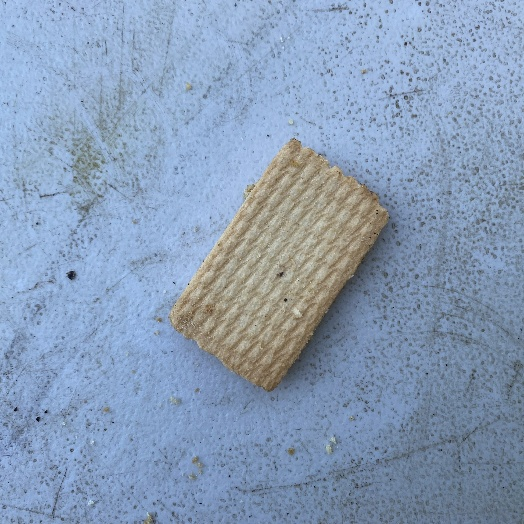
\includegraphics[width=\linewidth]{figures/fig4_sample1.jpg}\\[2pt]
\footnotesize (a)
\end{minipage}\hfill
\begin{minipage}{0.30\linewidth}\centering
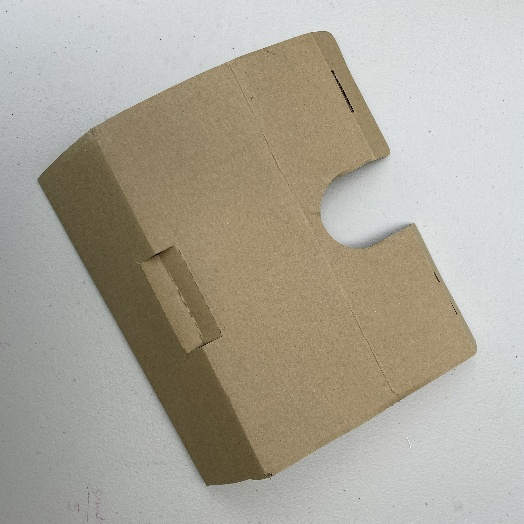
\includegraphics[width=\linewidth]{figures/fig4_sample2.jpg}\\[2pt]
\footnotesize (b)
\end{minipage}\hfill
\begin{minipage}{0.30\linewidth}\centering
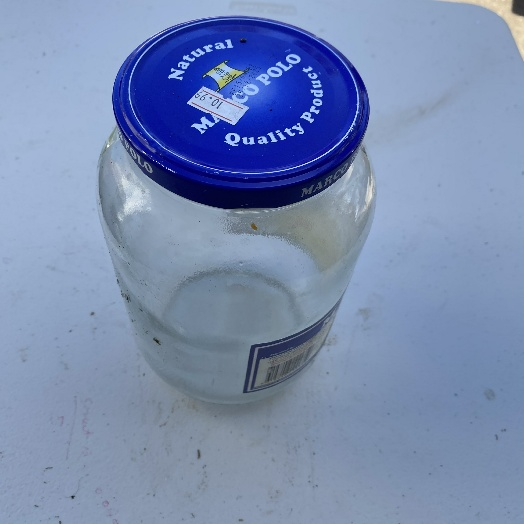
\includegraphics[width=\linewidth]{figures/fig4_sample3.jpg}\\[2pt]
\footnotesize (c)
\end{minipage}\\
\begin{minipage}{0.30\linewidth}\centering
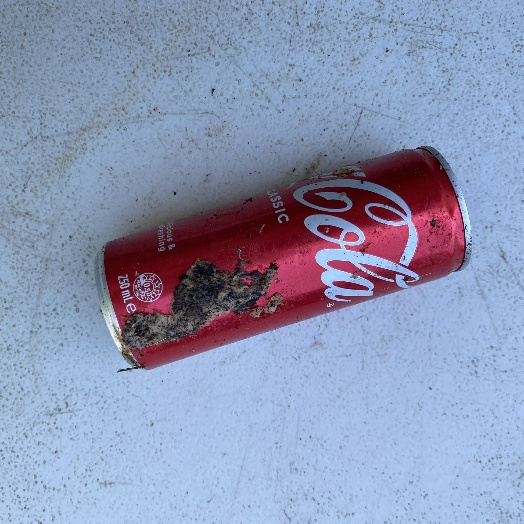
\includegraphics[width=\linewidth]{figures/fig4_sample4.jpg}\\[2pt]
\footnotesize (d)
\end{minipage}\hfill
\begin{minipage}{0.30\linewidth}\centering
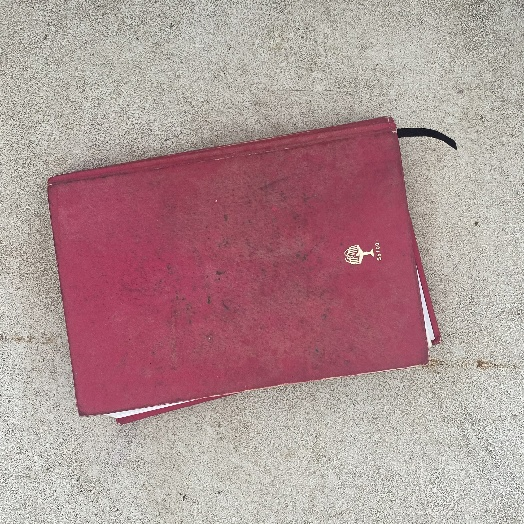
\includegraphics[width=\linewidth]{figures/fig4_sample5.jpg}\\[2pt]
\footnotesize (e)
\end{minipage}\hfill
\begin{minipage}{0.30\linewidth}\centering
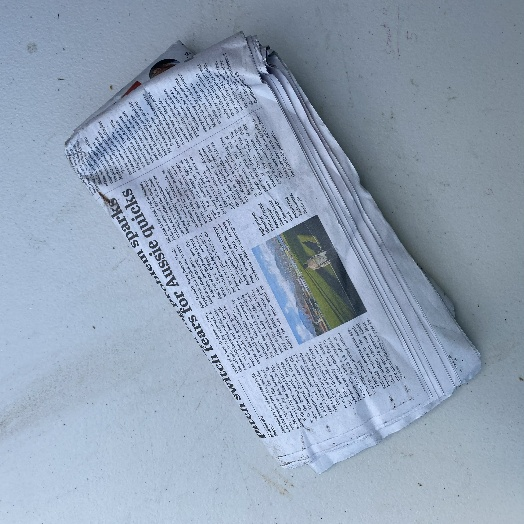
\includegraphics[width=\linewidth]{figures/fig4_sample6.jpg}\\[2pt]
\footnotesize (f)
\end{minipage}\\
\begin{minipage}{0.30\linewidth}\centering

\includegraphics[width=\linewidth]{figures/fig4_sample7.jpg}\\[2pt]
\footnotesize (g)
\end{minipage}\hfill
\begin{minipage}{0.30\linewidth}\centering
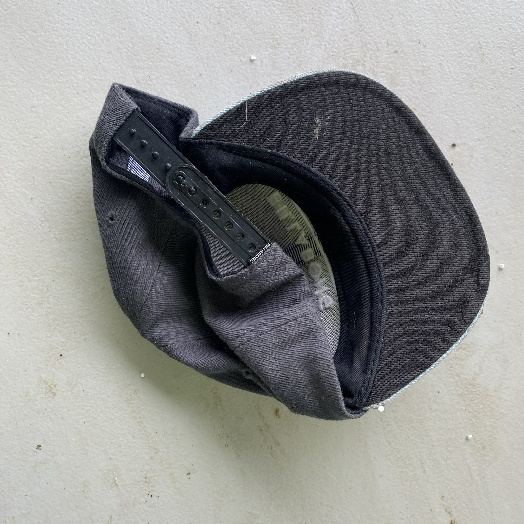
\includegraphics[width=\linewidth]{figures/fig4_sample8.jpg}\\[2pt]
\footnotesize (h)
\end{minipage}\hfill
\begin{minipage}{0.30\linewidth}\centering
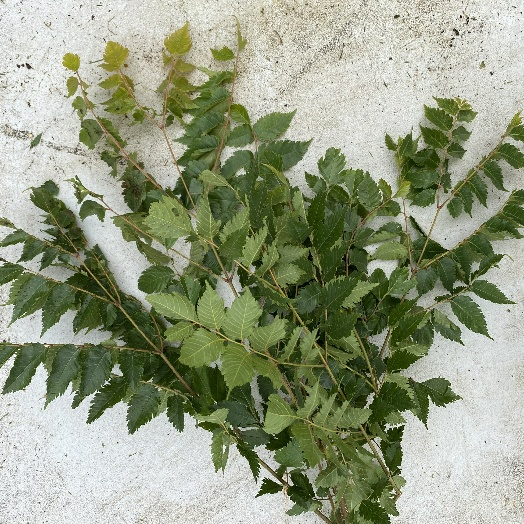
\includegraphics[width=\linewidth]{figures/fig4_sample9.jpg}\\[2pt]
\footnotesize (i)
\end{minipage}
\end{center}
\captionof{figure}{Representative samples of the nine waste classes of the RealWaste
dataset: (a)~Food Organics, (b)~Cardboard, (c)~Glass, (d)~Metal,
(e)~Miscellaneous Trash, (f)~Paper, (g)~Plastic, (h)~Textile Trash, and
(i)~Vegetation. Note the realistic, contaminated and visually ambiguous
conditions under which the images were captured.}
\label{fig:samples}

The dataset is partitioned into training (70\%), validation (15\%) and test
(15\%) sets using \emph{stratified} random splitting, which preserves the
relative class frequencies in every partition and yields 3{,}326 training,
713 validation and 713 test samples. Stratified splitting ensures that the
imbalance present in the raw data is mirrored and therefore explicitly
handled in all three partitions. Visual inspection confirmed that the
dataset is free of missing values and label inconsistencies.

\begin{center}
\begin{minipage}{0.49\linewidth}\centering
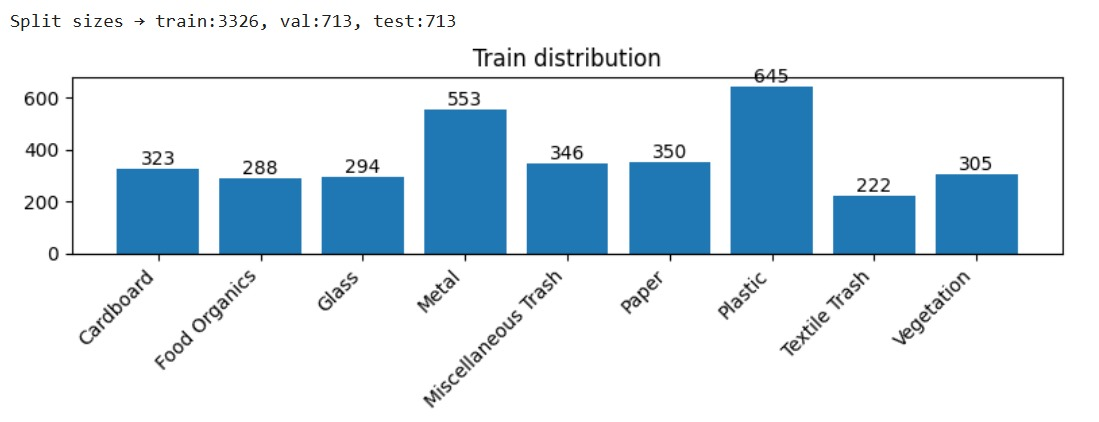
\includegraphics[width=\linewidth]{figures/fig5_dist_train.jpg}\\[2pt]
\footnotesize Training (3{,}326 images)
\end{minipage}\hfill
\begin{minipage}{0.49\linewidth}\centering
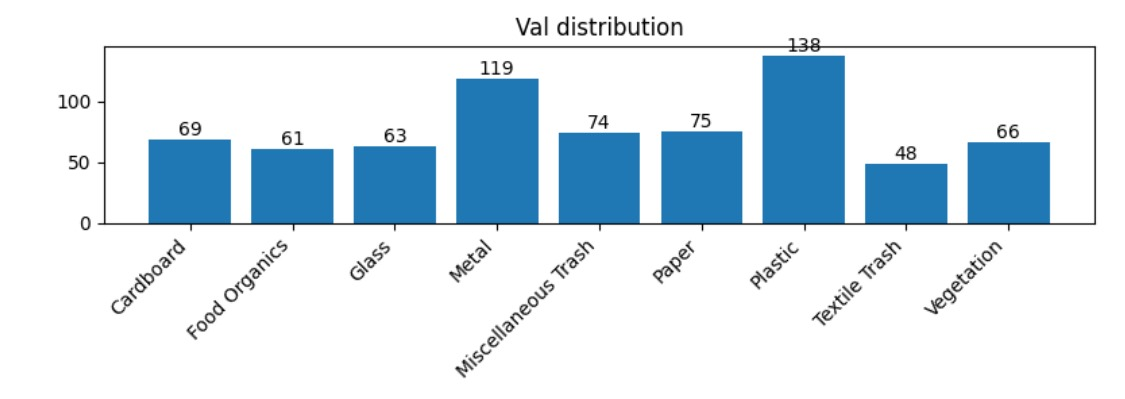
\includegraphics[width=\linewidth]{figures/fig5_dist_val.jpg}\\[2pt]
\footnotesize Validation (713 images)
\end{minipage}\\
\begin{minipage}{0.49\linewidth}\centering
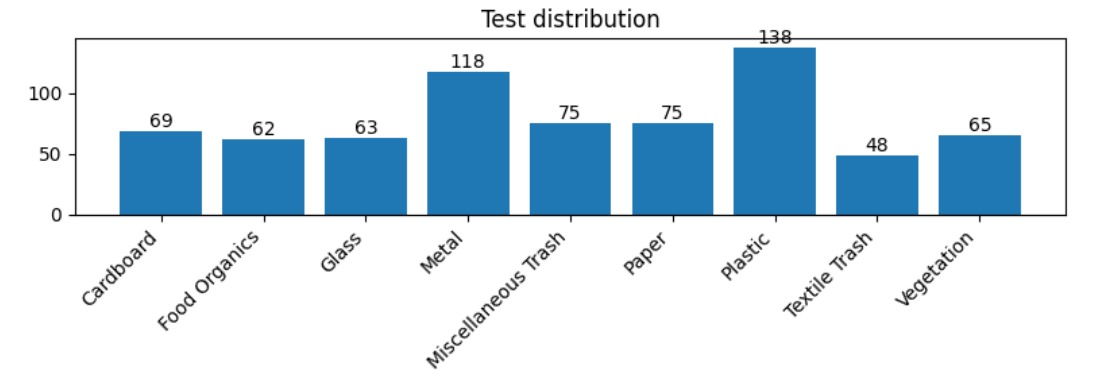
\includegraphics[width=\linewidth]{figures/fig5_dist_test.jpg}\\[2pt]
\footnotesize Test (713 images)
\end{minipage}
\end{center}
\captionof{figure}{Class distribution of the training, validation and test partitions
after stratified 70/15/15 splitting. Every partition preserves the relative
frequencies of the nine classes.}
\label{fig:distribution}

As real landfill images are captured under heterogeneous lighting, scale and
orientation conditions, the train and test pipelines differ appropriately.
For the training split we apply the augmentation operators
\begin{align}
  \text{(a)}&\ \text{RandomResizedCrop}(224),\\
  \text{(b)}&\ \text{RandomHorizontalFlip}(),
\end{align}
which introduce scale, aspect-ratio and mirroring variability and act as
regularisers for the imbalanced data. The validation and test sets instead
use the deterministic pipeline Resize(256) (short side) followed by
CenterCrop(224). In all cases the resized images are converted to tensors and
normalised with the ImageNet statistics
$\boldsymbol\mu=\{0.485,0.456,0.406\}$ and
$\boldsymbol\sigma=\{0.229,0.224,0.225\}$. Figure~\ref{fig:augmentation}
illustrates the effect of the augmentation operators on a representative
sample.

\begin{center}
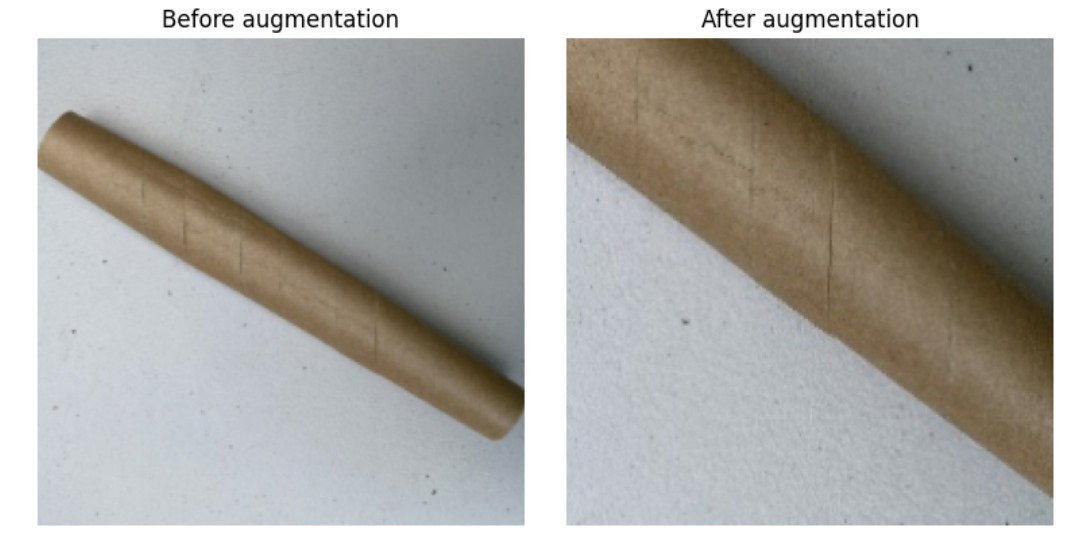
\includegraphics[width=0.9\linewidth]{figures/fig6_augmentation.jpg}
\end{center}
\captionof{figure}{Data augmentation applied to the training split. The operators
introduce scale, aspect-ratio and mirroring variability that regularise the
learning process on the imbalanced dataset.}
\label{fig:augmentation}

\subsection{Overall framework}\label{sec:framework}

Figure~\ref{fig:methodology} outlines the proposed pipeline, which comprises
three phases: (i)~preprocessing, (ii)~training, and (iii)~testing. During
preprocessing, raw landfill images are loaded, resized to the backbone input
resolution, and split stratifiedly as described in
Section~\ref{sec:dataset}. During training, a pretrained backbone with frozen
convolutional parameters extracts feature maps; a channel-attention gate
recalibrates the final feature maps; and a newly initialised classifier head
maps the recalibrated representations to class probabilities. Only the
attention module and the classifier parameters are updated, while the
backbone remains fixed a protocol that preserves the pretrained
representations and enables fair comparisons across architectures. During
testing, the best-performing checkpoint (selected by validation accuracy) is
restored and evaluated on the unseen test set, and Grad-CAM heatmaps are
computed for qualitative analysis.

\begin{center}
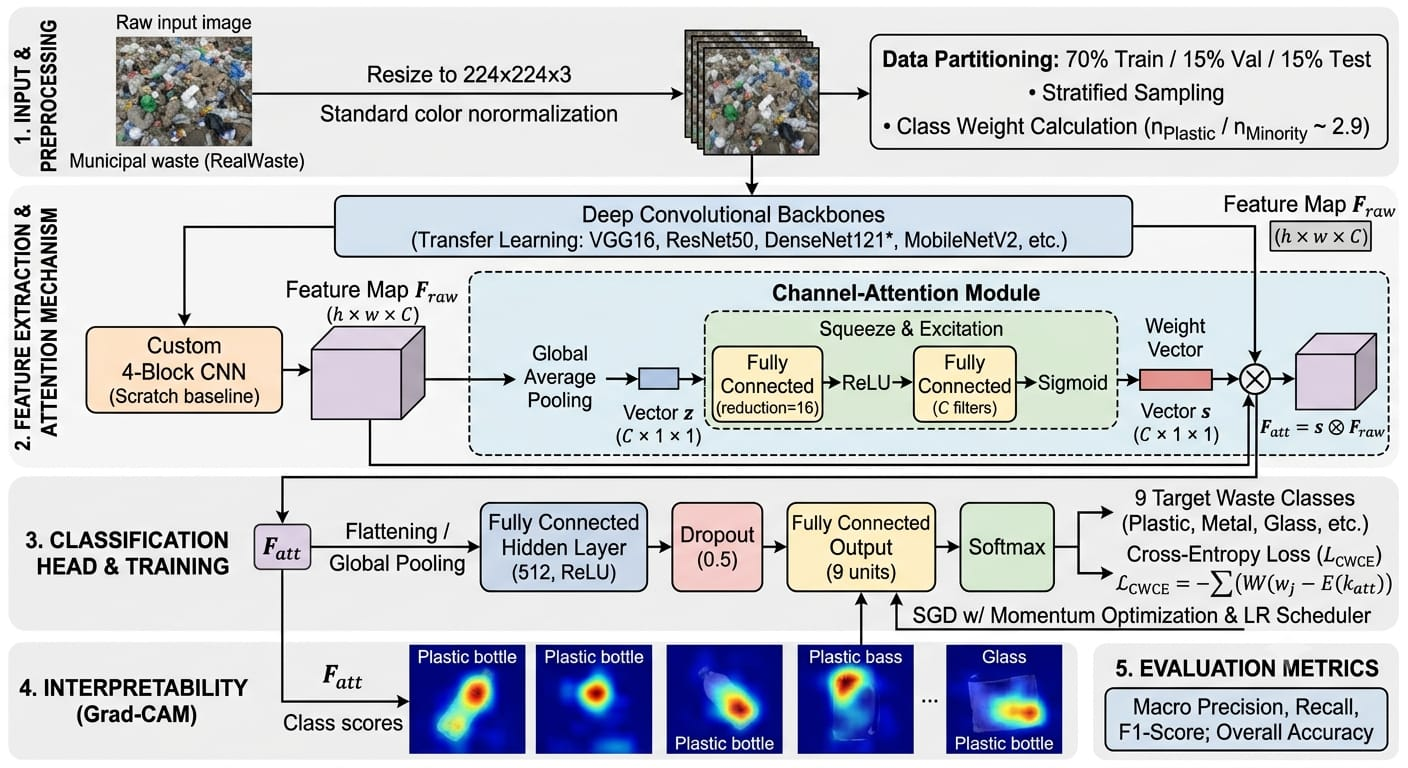
\includegraphics[width=\linewidth]{figures/fig2_methodology.jpeg}
\end{center}
\captionof{figure}{Proposed methodological pipeline. The preprocessing phase loads,
resizes and stratifies the raw landfill images; the training phase first
performs backbone feature extraction, then channel-attention recalibration
and classification, updating only the attention and classifier parameters;
the testing phase restores the best checkpoint and produces predictions
together with Grad-CAM heatmaps.}
\label{fig:methodology}

\subsection{Channel attention module}\label{sec:channel-attention}

The core of the proposed framework is a lightweight channel-attention gate
(Figure~\ref{fig:attention}) that re-weights the feature maps computed by the
frozen backbone. Let
$\mathbf{X}\in\mathbb{R}^{C\times H \times W}$ denote the final convolutional
feature maps of the backbone, where $C$, $H$ and $W$ are the number of
channels, the height and the width, respectively. For DenseNet-121 these maps
are of size $1024\times7\times7$.

The gate first aggregates each channel plane into scalar descriptors using
two complementary pooling operators global average pooling, which encodes
the overall channel statistics, and global maximum pooling, which captures
the most discriminative response:

\begin{equation}\label{eq:gap}
  z^{\text{avg}}_c \;=\;
  \frac{1}{H\, W} \sum_{i=1}^{H}\sum_{j=1}^{W} X_c(i,j),
\end{equation}

\begin{equation}\label{eq:gmp}
  z^{\text{max}}_c \;=\;
  \max_{i\in[1,H],\, j\in[1,W]} X_c(i,j),
\end{equation}

with $\mathbf{z}^{\text{avg}}=[z^{\text{avg}}_1,\dots,z^{\text{avg}}_C]^\top$
and $\mathbf{z}^{\text{max}}=[z^{\text{max}}_1,\dots,z^{\text{max}}_C]^\top$.
The two descriptors are concatenated along the channel dimension,
$\mathbf{z}=[\mathbf{z}^{\text{avg}};\,\mathbf{z}^{\text{max}}]\in\mathbb{R}^{2C}$,
and passed through a bottleneck perceptron composed of a dimensionality
reduction layer (reduction ratio $r=16$), a ReLU activation
$\delta(\cdot)$, an expansion layer, and a sigmoid activation
$\sigma(\cdot)$. The resulting gate vector
$\mathbf{s}=[s_1,\dots,s_C]^\top\in(0,1)^C$ is

\begin{equation}\label{eq:attweights}
  \mathbf{s} \;=\;
  \sigma\!\Big(
    \mathbf{W}_2\; \delta\!\big( \mathbf{W}_1 \mathbf{z} \big)
  \Big),
\end{equation}

where $\mathbf{W}_1 \in \mathbb{R}^{(C/r)\times 2C}$ and
$\mathbf{W}_2 \in \mathbb{R}^{C \times (C/r)}$ are learnable weight matrices.
Finally, each channel of the feature map is re-scaled by its corresponding
gate value:

\begin{equation}\label{eq:recalib}
  \widetilde{\mathbf{X}}_c \;=\; s_c \odot \mathbf{X}_c,
\qquad c = 1,\dots,C,
\end{equation}

where $\odot$ denotes element-wise multiplication and the scalar $s_c$ is
broadcast over the spatial dimensions. This recalibration is applied to the
\emph{final} feature maps of the backbone, immediately before the classifier
head, and is therefore fully differentientiable and trainable from
scratch. The attention mechanism is applied in the same way for each of the
backbones studied in Section~\ref{sec:results}, so that the only
architecture-dependent quantities are the number of channels $C$ and, for
Inception-based models, the input resolution (Table~\ref{tbl:backbones}).

\begin{center}
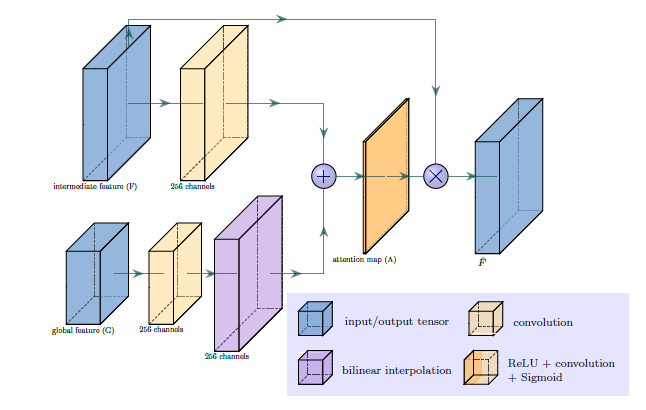
\includegraphics[width=0.9\linewidth]{figures/fig3_attention.png}
\end{center}
\captionof{figure}{Structure of the channel-attention gate. The final feature maps are
pooled with global average and maximum pooling, concatenated, and passed
through a two-layer bottleneck perceptron followed by a sigmoid activation;
the resulting gate vector recalibrates the feature maps channel-wise.}
\label{fig:attention}

\begin{table}[t]
\small
\rmfamily
\caption{Backbone configurations used for transfer learning. In all cases the
convolutional body is frozen and only the attention module and the classifier
are trained. \tsc{SE} denotes the channel-attention gate of
Section~\ref{sec:channel-attention}.}
\label{tbl:backbones}
\begin{tabular*}{\tblwidth}{@{\extracolsep{\fill}} lcc @{}}
\toprule
Model & Input size & Final channels\\
\midrule
VGG-16 & $224\times224$ & 512\\
ResNet-50 & $224\times224$ & 2048\\
MobileNetV2 & $224\times224$ & 1280\\
\textbf{DenseNet-121} & \textbf{$224\times224$} & \textbf{1024}\\
Inception-v3 & $299\times299$ & 2048\\
Inception-ResNet-v2 & $299\times299$ & 1536\\
Custom CNN & $224\times224$ & 256\\
\bottomrule
\end{tabular*}
\end{table}

\subsection{DenseNet-121 backbone}\label{sec:densenet}

We select DenseNet-121~\cite{huang_densenet} as the primary backbone of the
proposed framework. Dense convolutional networks connect each layer to every
other layer within a dense block, promoting maximal feature reuse,
mitigating the vanishing-gradient problem and reducing the parameter count
compared with equally deep ResNet architectures. These properties are
particularly attractive for a small and heterogeneous dataset such as
RealWaste, where the capacity to recombine features at multiple depths is
more valuable than brute-force depth. The 121-layer variant ends with a
transition block that produces $1024\times7\times7$ feature maps, which are
recalibrated by the channel-attention gate
(Section~\ref{sec:channel-attention}), flattened, and mapped to the $K=9$
class logits by the classifier head. The convolutional parameters are kept
frozen to preserve ImageNet knowledge and to keep the number of trainable
parameters small; only the attention gate and the classifier
($\approx
0.15$M parameters) are updated during training.

\subsection{Training strategy}\label{sec:training}

Because the class distribution is strongly imbalanced, a plain
cross-entropy objective would bias the model towards the majority classes. We
therefore minimise the class-weighted cross-entropy loss

\begin{equation}\label{eq:loss}
  \mathcal{L}(\boldsymbol\theta) \;=\;
  -\,\frac{1}{N}\sum_{n=1}^{N} w_{y_n}\; \log p_{y_n}(\mathbf{x}_n),
\qquad
  w_c \;=\; \frac{N}{K\, n_c},
\end{equation}

where $n_c$ is the number of training samples of class $c$ and $N$ is the
total number of training samples. The weighting $w_c$ is inversely
proportional to the class frequency and restores the balance of the effective
gradient contributions of minority classes without altering the sample
distribution~\cite{cui_classbalanced}.

The objective~\eqref{eq:loss} is optimised with the Adam
optimiser~\cite{kingma_adam} (initial learning rate $10^{-3}$, batch size
$32$). A \emph{ReduceLROnPlateau} scheduler monitors the validation loss and,
when no improvement is observed for two consecutive epochs, reduces the
learning rate by a factor of $0.1$; this dynamic adaptation is essential for
such small datasets, where a fixed learning rate either stalls early or
oscillates~\cite{goyal_bigbatch}. Early stopping with a patience of five
epochs (monitored on validation loss) prevents overfitting, and the model
checkpoint that achieves the highest validation accuracy is retained for final
evaluation. All random seeds are fixed (seed $=42$) for Python, NumPy and
PyTorch to guarantee reproducibility~\cite{paszke_pytorch}. Table~\ref{tbl:hyperparams}
summarises the hyperparameters.

\begin{table}[t]
\small
\rmfamily
\caption{Training hyperparameters of the proposed framework.}
\label{tbl:hyperparams}
\begin{tabular*}{\tblwidth}{@{\extracolsep{\fill}} ll @{}}
\toprule
Hyperparameter & Setting\\
\midrule
Backbone & DenseNet-121 (frozen ImageNet weights)\\
Trainable modules & Channel attention + classifier\\
Optimiser & Adam\\
Initial learning rate & $1\times10^{-3}$\\
Batch size & 32\\
Maximum epochs & 50\\
LR scheduler & ReduceLROnPlateau ($0.1$, patience 2)\\
Early stopping & Patience 5 (validation loss)\\
Loss & Class-weighted cross-entropy \eqref{eq:loss}\\
Checkpointing & Best validation accuracy\\
Input resolution & $224\times224$\\
Normalisation & ImageNet mean/std\\
Random seed & 42\\
\bottomrule
\end{tabular*}
\end{table}

\subsection{Evaluation metrics and explainability}\label{sec:evaluation}

Let $\mathrm{TP}_c$, $\mathrm{FP}_c$ and $\mathrm{FN}_c$ denote the number of
true positives, false positives and false negatives of class $c$ on the test
set. Per-class precision, recall and $F_1$-score, along with the global
accuracy, are defined as

\begin{align}
  P_c &= \frac{\mathrm{TP}_c}{\mathrm{TP}_c + \mathrm{FP}_c},
  \qquad R_c = \frac{\mathrm{TP}_c}{\mathrm{TP}_c + \mathrm{FN}_c},\\
  F_{1,c} &= \frac{2\, P_c\, R_c}{P_c + R_c},
  \qquad \mathrm{Acc} = \frac{1}{N_{\text{test}}}\sum_{c=1}^{K} \mathrm{TP}_c,
\end{align}

where $N_{\text{test}}$ is the size of the test set. Macro-averaged scores
are obtained by averaging the per-class values. We report accuracy together
with macro precision, recall and $F_1$ for the backbone comparison, and the
full per-class reports for the ablation study.

For interpretability we employ gradient-weighted class activation
mapping~\cite{selvaraju_gradcam}. Let $\mathbf{A}^k$ denote the $k$-th
feature plane of the (post-attention) target feature maps and let $y^{c}$ be
the logit (score) of the predicted class $c$. The neuron importance weights
are obtained by global-average-pooling the gradients of $y^c$ with respect
to the feature planes:

\begin{equation}\label{eq:gradcamw}
  \alpha_k^{c} \;=\;
  \frac{1}{Z}\sum_{i=1}^{H}\sum_{j=1}^{W}
  \frac{\partial y^{c}}{\partial A^{k}_{ij}},
\end{equation}

where $Z = H\cdot W$ is the number of spatial locations. The class-specific
saliency map is

\begin{equation}\label{eq:gradcamm}
  L^{c}_{\text{Grad-CAM}}(i,j) \;=\;
  \mathrm{ReLU}\!\left(\sum_{k=1}^{C} \alpha_k^{c}\; A^{k}_{ij}\right),
\end{equation}

which is up-sampled to the input resolution and overlaid on the original
image. The ReLU keeps only the features whose gradients are positively
correlated with the class score, highlighting the regions that support the
prediction.

\section{Results and Discussion}\label{sec:results}

\subsection{Implementation details}

The framework is implemented in Python with PyTorch~\cite{paszke_pytorch} and
torchvision. Pretrained weights are taken from the ImageNet-1K checkpoints
distributed with torchvision; DenseNet-121 is loaded with
\verb|weights=models.DenseNet121_Weights.IMAGENET1K_V1|. Inception-ResNet-v2
is provided via the \emph{timm} library. The channel-attention gate uses a
reduction ratio of $16$ and is instantiatted per backbone with the number of
channels shown in Table~\ref{tbl:backbones}. All experiments are run on a
single NVIDIA GPU. The training loop follows Section~\ref{sec:training},
with the best checkpoint selected by validation accuracy and restored for the
final test evaluation. Stochastic data loading, batching and class-weighted
loss are applied identically to all models.

\subsection{Comparison with pretrained backbones}\label{sec:backbone}

Table~\ref{tbl:comparison} compares the proposed attention-gated DenseNet-121
with the six competing backbones on the common test set. DenseNet-121 yields
the strongest results, achieving an accuracy of $0.82$ and macro precision,
recall and $F_1$ of $0.83$, $0.83$ and $0.83$, respectively. ResNet-50
(accuracy $0.79$) and MobileNetV2 (accuracy $0.78$) follow closely and offer
a favourable accuracy--efficiency trade-off, whereas the compact custom CNN
is competitive ($0.77$) but is limited by the absence of large-scale
pretraining. VGG-16 and the Inception family saturate in the mid-$0.74$--$0.75$
range. The consistent advantage of DenseNet-121 suggests that dense
connectivity, together with channel attention, provides the most robust
feature representations for authentic waste imagery under identical data and
optimisation conditions. The learning curves of the proposed model
(Figure~\ref{fig:learning}) show a smooth and stable convergence: the
training and validation losses decrease monotonically with modest
fluctuations, and the validation accuracy plateaus at a high level, the
hallmark of a well-regularised model.

\begin{center}
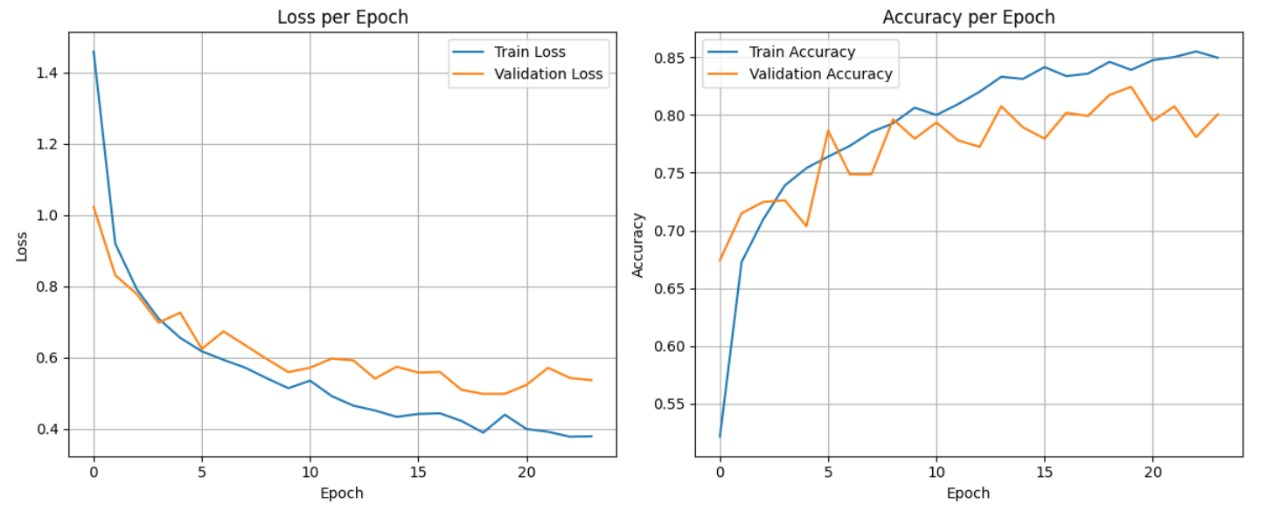
\includegraphics[width=0.9\linewidth]{figures/fig7_learning_densenet.jpg}
\end{center}
\captionof{figure}{Training and validation curves of the proposed attention-guided
DenseNet-121 model. The losses decrease monotonically and the validation
accuracy converges to a stable plateau, indicating well-regulated training
without overfitting.}
\label{fig:learning}

\begin{table*}[t]
\small
\rmfamily
\caption{Test performance (top-1 accuracy and macro-averaged precision,
recall and $F_1$-score) of the seven attention-gated backbones on the
RealWaste test set. The proposed DenseNet-121 framework performs best.}
\label{tbl:comparison}
\begin{tabular*}{\tblwidth}{@{\extracolsep{\fill}} lcccc @{}}
\toprule
Model (with channel attention) & Accuracy & Macro Precision & Macro Recall & Macro $F_1$\\
\midrule
\textbf{DenseNet-121 (proposed)} & \textbf{0.82} & \textbf{0.83} & \textbf{0.83} & \textbf{0.83}\\
ResNet-50   & 0.79 & 0.79 & 0.80 & 0.80\\
MobileNetV2 & 0.78 & 0.78 & 0.80 & 0.78\\
Custom CNN  & 0.77 & 0.77 & 0.78 & 0.77\\
VGG-16      & 0.75 & 0.76 & 0.76 & 0.75\\
Inception-ResNet-v2 & 0.74 & 0.74 & 0.75 & 0.74\\
Inception-v3 & 0.74 & 0.74 & 0.76 & 0.75\\
\bottomrule
\end{tabular*}
\end{table*}

\subsection{Ablation study: effect of channel attention}\label{sec:ablation}

\begin{table*}[t]
\small
\rmfamily
\caption{Per-class precision ($P$), recall ($R$) and $F_1$-score of
DenseNet-121 with and without the channel-attention gate on the RealWaste
test set. The attention mechanism raises the overall accuracy from
79.41\% to 82.35\% and the macro-$F_1$ from 0.80 to 0.83.}
\label{tbl:ablation}
\begin{tabular*}{\tblwidth}{@{\extracolsep{\fill}} l ccc ccc @{}}
\toprule
 & \multicolumn{3}{c}{Without attention} & \multicolumn{3}{c}{With attention (proposed)}\\
\cmidrule(lr){2-4}\cmidrule(lr){5-7}
Class & $P$ & $R$ & $F_1$ & $P$ & $R$ & $F_1$\\
\midrule
Cardboard           & 0.88 & 0.71 & 0.78 & 0.90 & 0.87 & 0.89\\
Food Organics       & 0.82 & 0.89 & 0.85 & 0.89 & 0.87 & 0.88\\
Glass               & 0.92 & 0.88 & 0.85 & 0.77 & 0.85 & 0.85\\
Metal               & 0.76 & 0.84 & 0.80 & 0.75 & 0.89 & 0.81\\
Miscellaneous Trash & 0.64 & 0.65 & 0.65 & 0.82 & 0.63 & 0.71\\
Paper               & 0.84 & 0.88 & 0.86 & 0.89 & 0.83 & 0.86\\
Plastic             & 0.71 & 0.76 & 0.74 & 0.81 & 0.69 & 0.75\\
Textile Trash       & 0.82 & 0.72 & 0.76 & 0.79 & 0.81 & 0.80\\
Vegetation          & 0.95 & 0.94 & 0.94 & 0.86 & 0.97 & 0.91\\
\midrule
Accuracy            & \multicolumn{3}{c}{0.7941} & \multicolumn{3}{c}{0.8235}\\
Macro $F_1$         & \multicolumn{3}{c}{0.80} & \multicolumn{3}{c}{0.83}\\
\bottomrule
\end{tabular*}
\end{table*}

To isolate the contribution of the channel-attention gate, we compare the
proposed model against a DenseNet-121 baseline in which the attention module
is removed and only the classifier head is trained (Table~\ref{tbl:ablation}).
The attention mechanism improves the test
accuracy from $79.41\%$ to $82.35\%$ and the macro-averaged $F_1$-score from
$0.80$ to $0.83$. The improvements are most pronounced for precisely the
categories that a plain CNN finds hardest. Cardboard recall rises from
$0.71$ to $0.87$ (with a corresponding $F_1$ gain from $0.78$ to $0.89$),
while the precision of Miscellaneous Trash increases from $0.64$ to $0.82$
and its $F_1$ from $0.65$ to $0.71$. Vegetation, already the strongest
category of the baseline, improves its recall from $0.94$ to $0.97$. These
results indicate that channel attention enables the network to emphasise the
feature channels that carry discriminative evidence for visually similar or
heterogeneous materials, in line with the observed behaviour of SE-style
recalibration in other tasks~\cite{hu_senet,woo_cbam}.

\subsection{Confusion-matrix analysis}\label{sec:confusion}

The confusion matrix of the proposed model on the test set is displayed in
Figure~\ref{fig:cm}. Materials with distinctive visual signatures Metal
(101 correct), Vegetation (68), Glass (63) and Cardboard (62) achieve strong
diagonal counts, reflecting the reflective, textured, transparent or sharp
appearance of these materials. By contrast, Plastic is the most frequently
misclassified category: fifteen Plastic instances are labelled as Metal and
thirteen as Glass, because bottle caps and clear polymer containers mimic
metallic and vitreous surfaces, respectively. Miscellaneous Trash, whose
definition is inherently heterogeneous, exhibits the lowest recall, with
errors spread across Plastic, Textile and Vegetation. Cardboard and Paper are
occasionally confused (three errors in each direction) owing to the visual
similarity of flattened printed packaging. Food Organics is nearly always
recognised, with a single misclassification, and Textile Trash is confused
with Metal and Miscellaneous Trash only rarely.

Taken together with the ablation (Section~\ref{sec:ablation}), the
confusion-matrix evidence shows that the channel attention gate substantially
reduces cross-category leakage for the visually confusable pairs (see
Figure~\ref{fig:cm}, right panel). The remaining errors are concentrated in
the inherently ambiguous boundary between Plastic, Glass and Metal, and in
the catch-all Miscellaneous class, suggesting directions for label
refinement and targeted augmentation.

\begin{center}
\begin{minipage}{0.48\linewidth}\centering
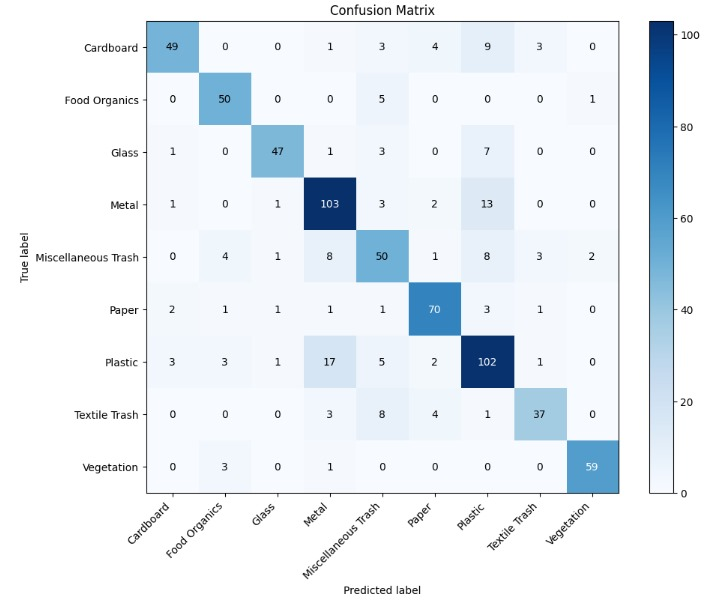
\includegraphics[width=\linewidth]{figures/fig9_cm_without_att.jpg}\\[2pt]
\footnotesize (a)~Without attention
\end{minipage}\hfill
\begin{minipage}{0.48\linewidth}\centering
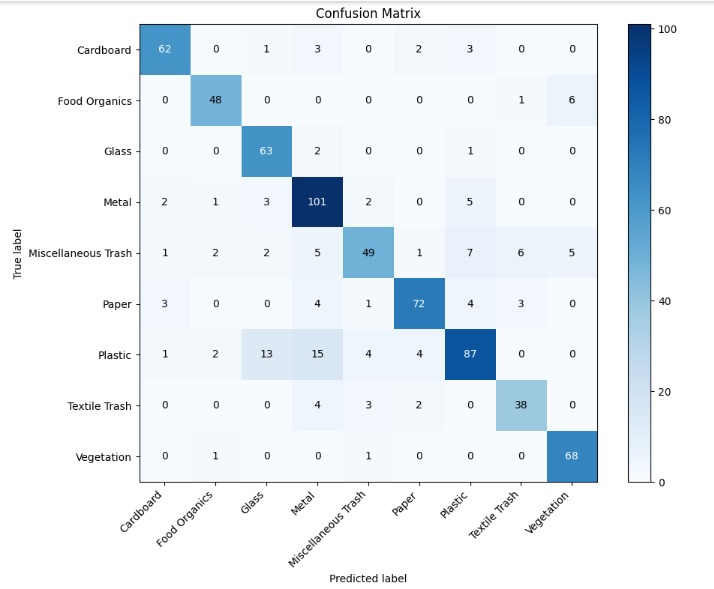
\includegraphics[width=\linewidth]{figures/fig9_cm_with_att.jpg}\\[2pt]
\footnotesize (b)~With attention (proposed)
\end{minipage}
\end{center}
\captionof{figure}{Confusion matrices of DenseNet-121 with and without the
channel-attention gate on the 713-image test set. The attention mechanism
reduces cross-category confusion, most notably between Cardboard and Paper
and between Plastic and Glass/Metal.}
\label{fig:cm}

\subsection{Grad-CAM explainability}\label{sec:gradcam}

Figure~\ref{fig:gradcam} presents Grad-CAM heatmaps for four representative
test images. In each case the activation map (right column) is overlaid on
the original photograph (left column). For the correctly classified
Vegetation sample, the heatmap is concentrated on the leaves and edges of
the plant, and the distracting background is suppressed evidence that the
model relies on salient, material-specific structure. The Miscellaneous
Trash item classified correctly focuses on the ribbed hoses, indicating
shape-based cues rather than texture. The two challenging examples are
equally informative: a Textile Trash sample is predicted as Miscellaneous
Trash because the model attends to stains and the circular weave pattern,
while a clear Glass shard is labelled as Metal because of its elongated,
specular reflection. These cases show that the model's errors are
\emph{comprehensible} and correspond to genuine visual ambiguities precisely
the kind of diagnostic insight that supports decision-making in operational
sorting facilities.

\begin{center}
\begin{minipage}{0.46\linewidth}\centering
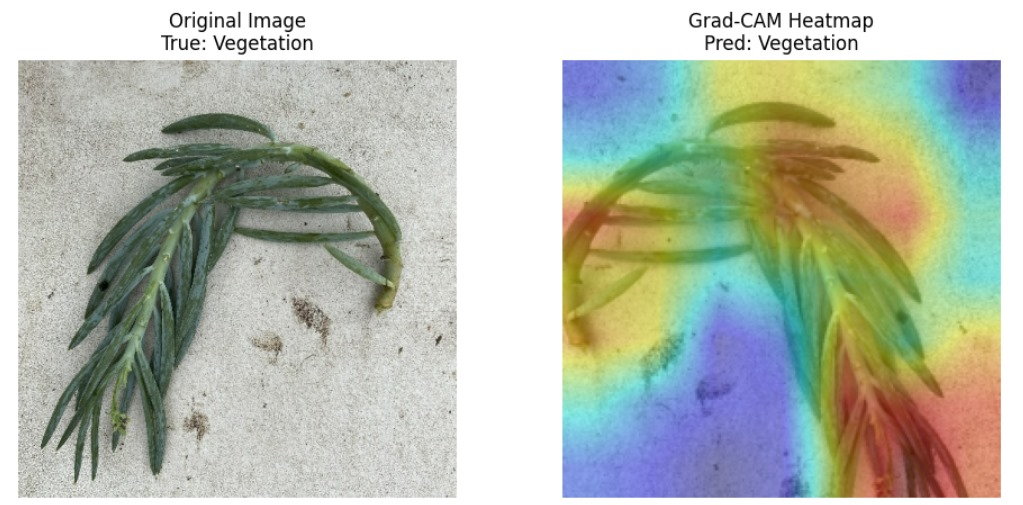
\includegraphics[width=\linewidth]{figures/fig10_gradcam_a.jpg}\\[2pt]
\footnotesize (a)~Vegetation $\rightarrow$ Vegetation (correct)
\end{minipage}\hfill
\begin{minipage}{0.46\linewidth}\centering
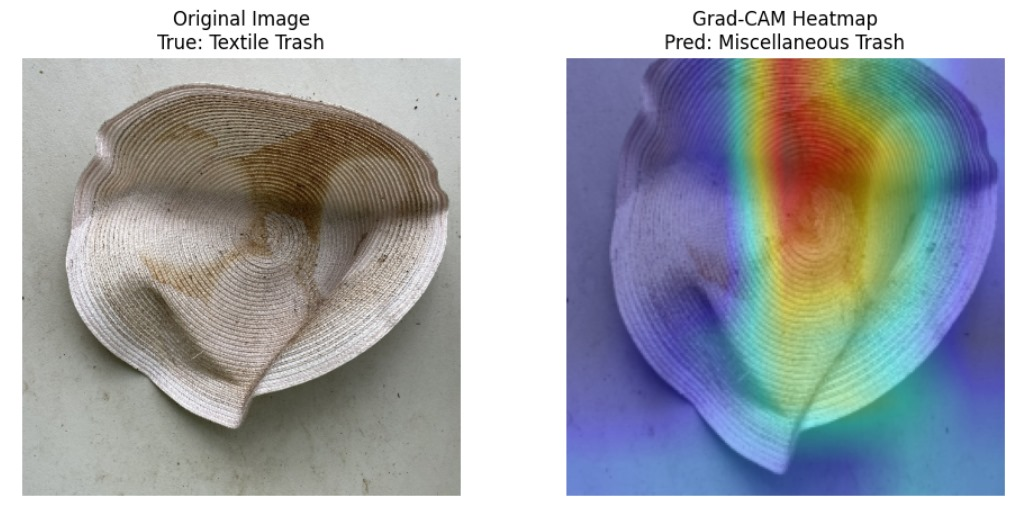
\includegraphics[width=\linewidth]{figures/fig10_gradcam_b.jpg}\\[2pt]
\footnotesize (b)~Miscellaneous $\rightarrow$ Miscellaneous Trash (correct)
\end{minipage}\\
\begin{minipage}{0.46\linewidth}\centering
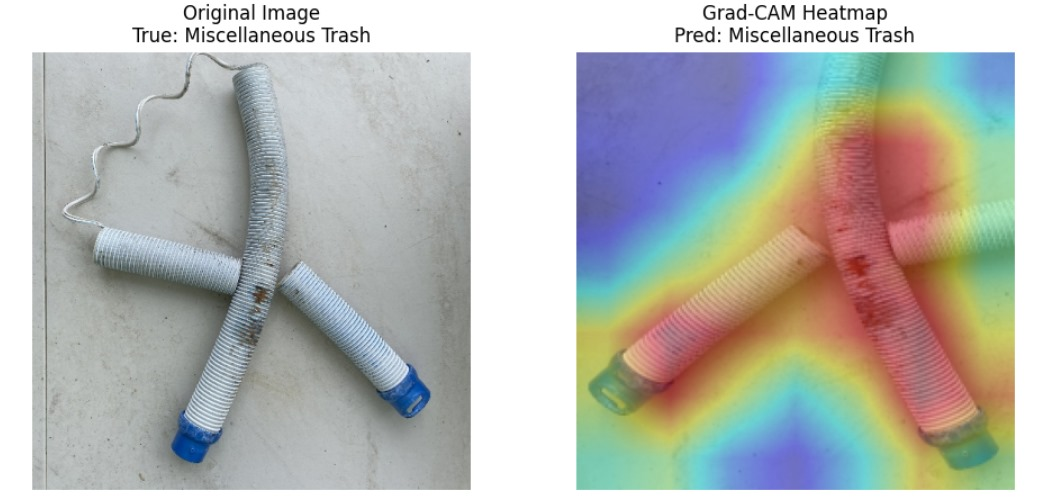
\includegraphics[width=\linewidth]{figures/fig10_gradcam_c.jpg}\\[2pt]
\footnotesize (c)~Textile $\rightarrow$ Miscellaneous Trash (wrong)
\end{minipage}\hfill
\begin{minipage}{0.46\linewidth}\centering
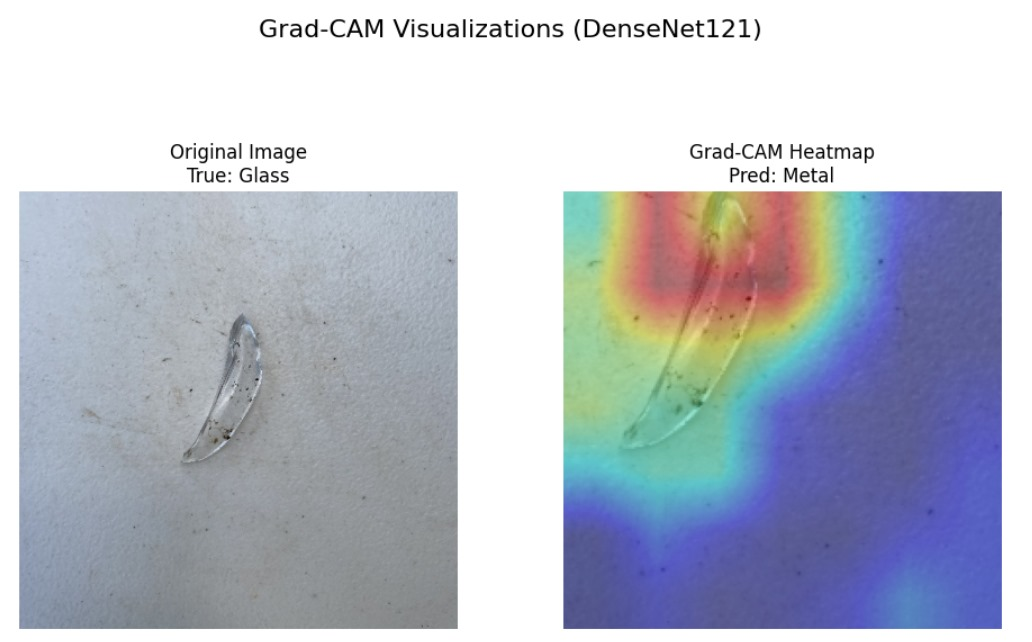
\includegraphics[width=\linewidth]{figures/fig10_gradcam_d.jpg}\\[2pt]
\footnotesize (d)~Glass $\rightarrow$ Metal (wrong)
\end{minipage}
\end{center}
\captionof{figure}{Grad-CAM explanations (overlay on the right of each panel) for four
representative test images. Correct predictions are localised on salient waste
objects, while the two misclassifications correspond to genuine visual
ambiguities detected by the model.}
\label{fig:gradcam}

\subsection{System deployment and web application}\label{sec:deployment}

To make the proposed framework practically usable, we package it into a
responsive web application that lets operators classify waste images through a
browser interface (Figure~\ref{fig:ui}). The application is built with the
\emph{Flask} web framework, which serves the front-end templates and manages
routing and user requests; the trained attention-guided DenseNet-121 model is
loaded in \emph{PyTorch} and performs inference on the server. Uploaded images
are preprocessed with \emph{TorchVision} (resize to $224\times224$,
normalisation with the ImageNet statistics of Section~\ref{sec:dataset}),
handled with \emph{Pillow}, and then forwarded to the model, which returns the
softmax probability vector over the nine waste classes. The front end is
implemented in HTML, CSS and JavaScript and communicates with the backend
through asynchronous requests, so that the classification result is displayed
without reloading the page.

The user interaction flow comprises four steps: (i)~\emph{image upload}, where
the user drags and drops an image or selects a file, with the upload area
providing an image preview for confirmation; (ii)~\emph{classification}, where
a ``Categorize'' button initially disabled and enabled only after a valid
image is selected submits the image to the server and a loading overlay with
a spinner and a ``Please wait...'' message is shown; (iii)~\emph{result
display}, where the uploaded image and the predicted waste category together
with its probability (or the full probability distribution) are presented side
by side; and (iv)~\emph{error handling}, where a modal dialog reports invalid
files or processing errors. The interface uses a green colour palette
(primary colour \#4CAF50) with rounded buttons and hover effects, a responsive
flexbox layout, and the Tiro Bangla typeface to support Bengali text, making
the application accessible to non-technical operators in recycling and
landfill-sorting facilities.

\begin{center}

\includegraphics[width=0.95\linewidth]{figures/fig11_ui.jpg}
\end{center}
\captionof{figure}{Screen capture of the deployed web application classifying a
Cardboard sample. The interface shows the uploaded image together with the
predicted waste category and its confidence, and follows the upload-classify-
display workflow described in the text.}
\label{fig:ui}

\subsection{Limitations}\label{sec:limitations}

Several limitations should be acknowledged. First, the RealWaste dataset,
while realistic, contains only 4{,}752 images, and categories such as Textile
Trash remain under-represented despite class-weighting; additional samples
or synthetic augmentation for minority classes would likely yield further
gains. Second, the ``Miscellaneous Trash'' label groups visually unrelated
objects, and its heterogeneous nature caps the achievable recall. Third, the
frozen-backbone regime, while efficient, prevents the attention signal from
propagating into the convolutional layers; end-to-end fine-tuning with
careful regularisation may extract additional performance. Finally, the
evaluation is limited to top-1 accuracy and macro-averaged metrics on a
single-site dataset; broader generalisation across different landfills and
recycling facilities remains to be established.

\section{Conclusion and Future Work}\label{sec:conclusion}

This paper presented an attention-guided transfer-learning framework for
real-world waste classification. By inserting a lightweight channel-attention
gate after the frozen feature extractor of DenseNet-121 and training
exclusively the attention and classifier modules with class-weighted
cross-entropy, an adaptive learning-rate scheduler and early stopping, the
proposed model achieves a test accuracy of $82.35\%$ and a macro-$F_1$ of
$0.83$ on the nine-class RealWaste dataset, outperforming six alternative
transfer-learning backbones under an identical protocol. An ablation study
attributed a gain of $2.94$ percentage points in accuracy (from $79.41\%$)
and $0.03$ in macro-$F_1$ to the channel-attention mechanism, with the
greatest improvements in the hardest categories (Cardboard, Miscellaneous
Trash and Vegetation). Confusion-matrix analysis identified the Plastic--
Glass--Metal boundary and the heterogeneous Miscellaneous class as the
main sources of residual error, and Grad-CAM visualisations confirmed that
correct predictions are driven by salient waste objects rather than
background cues.

Future work will pursue three directions: (i)~extending RealWaste (or
adapting the model) to additional landfill sites and finer material
subcategories, in order to reduce the ambiguity of the Miscellaneous class
and to test cross-site generalisation; (ii)~exploring self-attention and
transformer architectures, and heterogeneous sensor modalities such as
near-infrared or depth imagery, which are expected to disambiguate
materials beyond the visible spectrum; and (iii)~investigating semi-
and self-supervised pretraining on unlabelled waste imagery as well as
lightweight quantised variants for real-time edge deployment in automated
sorting plants. We believe that transparent, accurate and reproducible
classifiers of the type proposed here constitute a practical building block
for sustainable waste management and circular-economy automation.

%% -----------------------------------------------------------------
\section*{Acknowledgements}
The author gratefully acknowledges the Department of Computer Science and
Engineering, International Islamic University Chittagong, for supporting
this research.

\bigskip
\printcredits

%% Bibliography
\bibliographystyle{cas-model2-names}
\bibliography{refs}

\end{document}